\subsection{Runtime Monitoring}

RPTR provides runtime monitoring of a ROS system. To this end, the tool is able to collect parameter information in real time as parameter transactions occur. When collected, transactional data is stored in a MySQL database and is referenced by the RPTR tool or other third party (possibly non-ROS) systems. There are two primary components to the runtime monitoring system that powers RPTR: The first is a library exposed to instrumented ROS nodes that provides the definition to the functions that were substitutes during instrumentation. The second is a ROS node that subscribes to incoming parameter transaction data published by the instrumented nodes.

\subsubsection{RPTR Library}
A ROS node is given access to the RPTR library by simply adding a �depends� tag to its manifest.xml file and adding a simple header �include� statement to the node�s source. Then, the instrumented RPTR function calls may leverage the library to accomplish any and all parameter transactions. The primary accomplishment the library makes is publishing all parameter transactions to the RPTR ros node that monitors and stores them (as well as allowing parameter server interaction). There were several attempted approaches when creating this library, several of which failed. We first give an overview of two of these failures in an effort to provide support for our chosen method.

\textbf{Approach 1: One Primary Library Class}
This approach attempted to create one large library class and have its objects exist in the target node�s source files. While this approached served as good starting point, we soon realized that we were unable to define a node handle. Because our library class was being included as a header file, and objects of our library class were being created globally, we encountered a runtime failure when ROS located the node handle housed within the library.
This failure occurred because a ROS node handle cannot be declared prior to initialization of the node (which is accomplished with the �ros::init(...)� command). The initialization of a node occurs within the main method of its source, and global library objects were detected prior to the main method and by extension, the initialization procedure.

\textbf{Approach 2: Static Methods}
Our second approach attempted to use all static methods to avoid creating an object (that was in turn invoking its class�s constructor, which in turn attempted to create the node handle as described above). However, this method also failed. Everything that a static method calls or references must be static. Therefore, the node handle must be static, as well as the publisher. In order to initialize a static class member, one must do so outside of the class. As soon as we were outside of the static class, we were in the global space again, and ran into the same issue as before (a node handle was being created before the node�s initialization routine completed).
One might ask why we didn�t simply create a new publisher and new node handle within each method on the fly, thereby avoiding the aforementioned issues? Essentially, the node handle must persist in order to accomplish the publication. If it is created in a local scope, as soon as the scope is exited, the node handle and the publisher will be destroyed (without accomplishing the publication).

\textbf{Approach Three: Queue-Based System}
Our successful approach leverages two library classes, one class that queues up transactions and another that �harvests� them and publishes them to the RPTR ROS node. The first class is initialized as several objects, one in each .cpp file of the node�s source. These objects have distinct names to avoid conflicts at compile time. This class does not have a node handle, rather monitors each parameter server transaction, and places each transaction in its own queue.

The second class, the harvester, exists as one object and is declared directly after the node�s initialization procedure occurs (i.e. the line after �ros::init(...)�). Because it occurs after the initialization, it is allowed to have a node handle and by extension, a publisher. The harvester node periodically (currently 30 Hz, although this is adjustable) �harvests� the queues from the other objects, clears them, and publishes everything that existed in the queue. This approach has shown success, and has not yet failed during our experiments.

Note that after the transaction data has been published, the original parameter API call is allowed to execute. This ensures that the original behavior of the target system is not modified, because all original functionality is still taking place. RPTR is simply �stepping in� in the middle to copy and publish the data.

\subsubsection{RPTR ROS Node}
Parameter transactions are published to a topic that is consumed by the RPTR node. This node exists at runtime with the target system and is in charge of data-basing and verifying parameter transactions. When a transaction arrives, say a �GET� request, it is first verified for validity and then added to the database. Verification consists of ensuring that the request is legal. While much of the parameter analysis that RPTR provides is subjective and domain-specific (i.e. a developer must pose queries and analyze results), there are certain behaviors that are known to be incorrect, such as attempting to retrieve a parameter that has been deleted or does not exist. RPTR detects them and reports an alert to the user (as well as the database). In this way, we have enriched the default ROS functionality (ROS will not issue such warnings).

\begin{figure}
\begin{center}
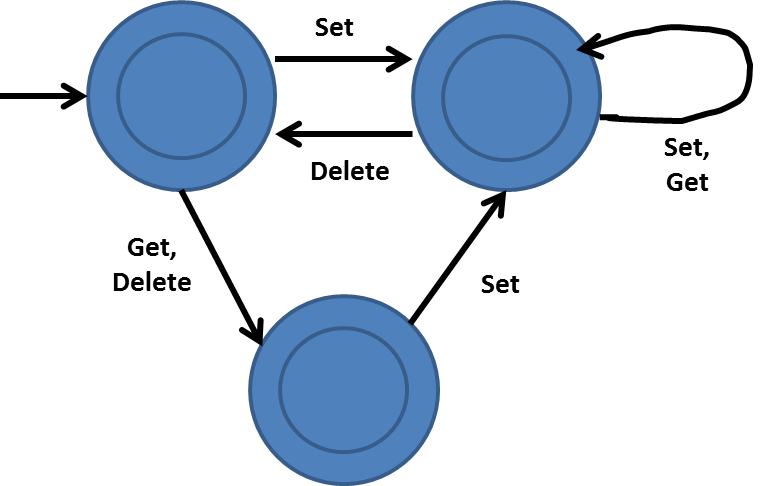
\includegraphics[scale=0.5]{images/statediagram}
\caption{Simple 3 State FSA for Verifying Parameter Transactions in the RPTR Node}
\end{center}
\end{figure}

In order to check for such errors, we make use of a simple state machine. The RPTR node queries the database in order to retrieve the most recent �state� of a given parameter, and then checks that the current requested operation does not lead the parameter into an error state. For example, if parameter �x� has been deleted, the only legal operations are to recreate (i.e. �SET�) x. If a node attempts to delete x, or get its value, then x will be led into an error state.

Note, the error state in this state machine is non-trapping, i.e. a parameter that was previously in an erroneous state is allowed to move to a legal state by making a legal transaction. For example, is x was deleted, and then deleted again, x would be in an error state. However, �setting� x would be legal, and x would move into a legal state. If we did not follow such an approach, and used a trapping error state, we would miss potentially miss other errors, because every transaction would be deemed erroneous after the first, thereby preventing us from differentiating from legal and illegal state changes.

\subsubsection{RPTR Front-End}
The RPTR front end is a command line tool that interacts with database created by the RPTR node during runtime and produces a report for a given parameter. This tool can be used either while the target system is running, or afterwards. If it used while the system is running, the report will simply contain data from the time of report generation backwards. In order to use the front-end tool, one simply specifies the parameter name, and a report is generated.

The analysis provided by the report includes creation information about the parameter, as well as a temporal view of how it existed during the run of the system. All GET, SET and DELETE transactions are listed, in chronological order, and detailed information is given about each transaction. This information includes the node that executed the transaction, the namespace used, the API used, the time the transaction occurred, etc. In addition, if an error occurred during runtime (see above), an alert message is displayed in the report.

\begin{figure}
\begin{center}
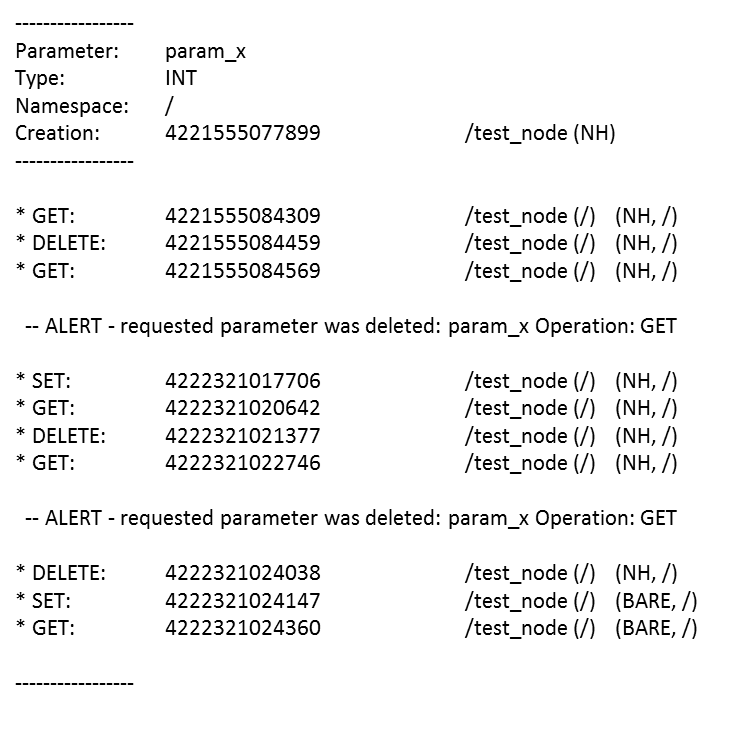
\includegraphics[scale=0.75]{images/samplereport}
\caption{An Example of a Report Generated by a Simple ROS System}
\end{center}
\end{figure}

We experimented with the idea of providing the end user with several different report options (i.e. only �GET� transactions, only �SET� transactions, etc.), however after evaluating the value of these various types of reports, we settled on only providing a comprehensive report. This allows the end user to have the most complete view of a parameter as it existed in the system during execution. Because of the modular design of the front-end, it would be simply to implement a custom report with custom metrics.
